\usetikzlibrary{calc}
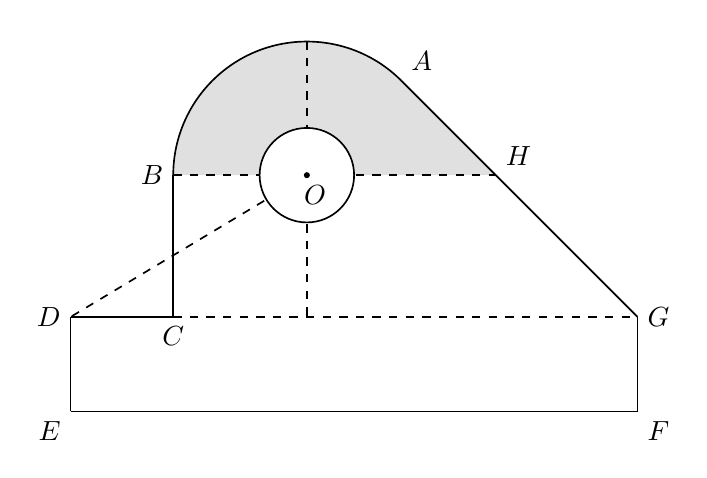
\begin{tikzpicture}[x=0.6cm,y=0.6cm,line width=.6pt,font=\normalsize]
% data units = cm; physical 0.6cm/unit -> body 72mm wide
\coordinate (E) at (0,0);
\coordinate (F) at (12,0);
\coordinate (G) at (12,2);
\coordinate (D) at (0,2);
\coordinate (O) at (5,5);
\coordinate (A) at (7,7);
\coordinate (C) at (2.1716,2);
\coordinate (B) at (2.1716,5);
\coordinate (H) at (9,5);
\coordinate (N) at (5,2);
\coordinate (T) at (5,7.8284);
% shaded region above B-H: H-A-arc-B
\fill[black!12] (H)--(A) arc[start angle=45,end angle=180,radius=1.6971cm]--cycle;
% contour solid
\draw (E)--(F)--(G);
\draw (E)--(D);
\draw (D)--(C);
\draw (C)--(B);
\draw (A) arc[start angle=45,end angle=180,radius=1.6971cm];
\draw (A)--(G);
% dashed construction / hidden
\draw[dashed] (C)--(G);
\draw[dashed] (B)--(H);
\draw[dashed] (T)--(N);
\draw[dashed] (O)--(D);
% hole: white interior, solid outline
\fill[white] (O) circle[radius=0.6cm];
\draw (O) circle[radius=0.6cm];
% center dot
\fill (O) circle[radius=1.1pt];
% labels in visible whitespace, offset from lines
\node[left] at (D) {$D$};
\node[below left] at (E) {$E$};
\node[below right] at (F) {$F$};
\node[right] at (G) {$G$};
\node[below] at (C) {$C$};
\node[left] at (B) {$B$};
\node[below,xshift=3pt] at (O) {$O$};
\node[above right] at (A) {$A$};
\node[above right] at (H) {$H$};
\end{tikzpicture}
